\documentclass[11pt]{article}

% ------------------------------------------------------------
% Standard LaTeX packages
% ------------------------------------------------------------
\usepackage[margin=1in]{geometry}
\usepackage{amsmath,amssymb,mathtools}
\usepackage{amsthm}
\usepackage[american]{babel}
\usepackage{stmaryrd}
\usepackage{enumitem}
\usepackage{booktabs}
\usepackage{array}
\usepackage{listings}
\usepackage[x11names,table]{xcolor}
\usepackage{mdframed}
\usepackage{tikz}
\usetikzlibrary{arrows.meta,positioning,calc,decorations.pathreplacing}
\usepackage{url}
\usepackage[colorlinks=true,linkcolor=blue,citecolor=blue,urlcolor=blue]{hyperref}

% ---------- Theorem environments ----------
\theoremstyle{plain}
\newtheorem{theorem}{Theorem}[section]
\newtheorem{proposition}[theorem]{Proposition}
\newtheorem{lemma}[theorem]{Lemma}
\newtheorem{corollary}[theorem]{Corollary}

\theoremstyle{definition}
\newtheorem{definition}[theorem]{Definition}
\newtheorem{axiombox}[theorem]{Axiom}
\newtheorem{protocol}[theorem]{Protocol}
\newtheorem{example}[theorem]{Example}

\theoremstyle{remark}
\newtheorem{remark}[theorem]{Remark}

% ---------- Lean repo link ----------
\newcommand{\leanRepo}{\url{https://doi.org/10.5281/zenodo.18779210}}

% ---------- Notation ----------
\newcommand{\N}{\mathbb{N}}
\newcommand{\Z}{\mathbb{Z}}
\newcommand{\Q}{\mathbb{Q}}
\newcommand{\R}{\mathbb{R}}
\newcommand{\C}{\mathbb{C}}
\newcommand{\F}{\mathbb{F}}
\newcommand{\Fp}{\mathbb{F}_p}
\newcommand{\Qbar}{\overline{\Q}}
\newcommand{\Qp}{\Q_p}
\newcommand{\Qell}{\Q_\ell}
\newcommand{\A}{\mathbb{A}}
\newcommand{\calO}{\mathcal{O}}
\newcommand{\fm}{\mathfrak{m}}
\newcommand{\fp}{\mathfrak{p}}
\newcommand{\Gal}{\mathrm{Gal}}
\newcommand{\GL}{\mathrm{GL}}
\newcommand{\Hom}{\mathrm{Hom}}
\newcommand{\Ext}{\mathrm{Ext}}
\newcommand{\CH}{\mathrm{CH}}
\newcommand{\cl}{\mathrm{cl}}
\newcommand{\End}{\mathrm{End}}
\newcommand{\Frob}{\mathrm{Frob}}
\newcommand{\CRM}{\mathrm{CRM}}
\newcommand{\tr}{\mathrm{tr}}
\newcommand{\rk}{\mathrm{rk}}
\newcommand{\NS}{\mathrm{NS}}
\newcommand{\Hdg}{\mathrm{Hdg}}

\newcommand{\BISH}{\mathsf{BISH}}
\newcommand{\LPO}{\mathsf{LPO}}
\newcommand{\WLPO}{\mathsf{WLPO}}
\newcommand{\LLPO}{\mathsf{LLPO}}
\newcommand{\MP}{\mathsf{MP}}
\newcommand{\FT}{\mathsf{FT}}
\newcommand{\CLASS}{\mathsf{CLASS}}

\newcommand{\CBN}{\mathrm{CBN}} % Classical Boundary Node

% ---------- Code listing style for Lean ----------
\definecolor{codegreen}{rgb}{0,0.6,0}
\definecolor{codegray}{rgb}{0.5,0.5,0.5}
\definecolor{codepurple}{rgb}{0.58,0,0.82}
\definecolor{backcolour}{rgb}{0.95,0.95,0.92}

\lstdefinelanguage{Lean}{
  keywords={theorem, lemma, def, definition, axiom, structure, class, instance,
            by, exact, intro, intros, apply, refine, constructor, use, obtain,
            have, show, from, fun, assume, let, in, if, then, else,
            match, with, end, namespace, section, variable, variables,
            example, begin, sorry, admit, noncomputable, classical,
            import, open, export, private, protected, mutual, meta,
            do, for, while, return, try, catch, finally,
            Type, Prop, Sort, Type*, forall, exists, where, extends,
            set, push_neg, rw, simp, omega, nlinarith, linarith,
            ext, rfl, congr, fin_cases, haveI, letI, attribute, inductive,
            deriving, opaque, decide, native_decide, abbrev},
  sensitive=true,
  morecomment=[l]{--},
  morecomment=[s]{/-}{-/},
  morestring=[b]",
  literate=
    {α}{{$\alpha$}}1 {β}{{$\beta$}}1 {γ}{{$\gamma$}}1
    {δ}{{$\delta$}}1 {ε}{{$\varepsilon$}}1 {ζ}{{$\zeta$}}1
    {η}{{$\eta$}}1 {θ}{{$\theta$}}1 {ι}{{$\iota$}}1
    {κ}{{$\kappa$}}1 {λ}{{$\lambda$}}1 {μ}{{$\mu$}}1
    {ν}{{$\nu$}}1 {ξ}{{$\xi$}}1 {π}{{$\pi$}}1
    {ρ}{{$\rho$}}1 {σ}{{$\sigma$}}1 {τ}{{$\tau$}}1
    {φ}{{$\varphi$}}1 {χ}{{$\chi$}}1 {ψ}{{$\psi$}}1
    {ω}{{$\omega$}}1 {Γ}{{$\Gamma$}}1 {Δ}{{$\Delta$}}1
    {Θ}{{$\Theta$}}1 {Λ}{{$\Lambda$}}1 {Σ}{{$\Sigma$}}1
    {Φ}{{$\Phi$}}1 {Ψ}{{$\Psi$}}1 {Ω}{{$\Omega$}}1
    {→}{{$\rightarrow$}}1 {←}{{$\leftarrow$}}1 {↔}{{$\leftrightarrow$}}1
    {⇒}{{$\Rightarrow$}}1 {⇐}{{$\Leftarrow$}}1 {⇔}{{$\Leftrightarrow$}}1
    {∀}{{$\forall$}}1 {∃}{{$\exists$}}1 {∈}{{$\in$}}1
    {∉}{{$\notin$}}1 {⊆}{{$\subseteq$}}1 {⊂}{{$\subset$}}1
    {∪}{{$\cup$}}1 {∩}{{$\cap$}}1 {≤}{{$\leq$}}1
    {≥}{{$\geq$}}1 {≠}{{$\neq$}}1 {≈}{{$\approx$}}1 {≃}{{$\simeq$}}1
    {≡}{{$\equiv$}}1 {∧}{{$\land$}}1 {∨}{{$\lor$}}1
    {¬}{{$\neg$}}1 {ℕ}{{$\mathbb{N}$}}1 {ℝ}{{$\mathbb{R}$}}1
    {ℂ}{{$\mathbb{C}$}}1 {ℤ}{{$\mathbb{Z}$}}1 {ℓ}{{$\ell$}}1
    {·}{{$\cdot$}}1 {∑}{{$\sum$}}1 {∏}{{$\prod$}}1
    {∅}{{$\emptyset$}}1 {∞}{{$\infty$}}1 {∂}{{$\partial$}}1
    {⟨}{{$\langle$}}1 {⟩}{{$\rangle$}}1 {…}{{$\ldots$}}1
    {₀}{{$_0$}}1 {₁}{{$_1$}}1 {₂}{{$_2$}}1 {⧸}{{$/$}}1 {‖}{{$\|$}}1
    {•}{{$\cdot$}}1 {⁻¹}{{$^{-1}$}}1 {⋆}{{$\star$}}1
    {∘}{{$\circ$}}1
    {×}{{$\times$}}1
    {ℚ}{{$\mathbb{Q}$}}1
}

\lstdefinestyle{leanstyle}{
    language=Lean,
    backgroundcolor=\color{backcolour},
    commentstyle=\color{codegreen},
    keywordstyle=\color{blue},
    stringstyle=\color{codepurple},
    basicstyle=\ttfamily\footnotesize,
    breakatwhitespace=false,
    breaklines=true,
    captionpos=b,
    keepspaces=true,
    numbers=left,
    numbersep=5pt,
    showspaces=false,
    showstringspaces=false,
    showtabs=false,
    tabsize=2,
    numberstyle=\tiny\color{codegray}
}

\lstset{style=leanstyle}

% ---------- Python listing style ----------
\lstdefinestyle{pythonstyle}{
    language=Python,
    backgroundcolor=\color{backcolour},
    commentstyle=\color{codegreen},
    keywordstyle=\color{blue},
    stringstyle=\color{codepurple},
    basicstyle=\ttfamily\footnotesize,
    breakatwhitespace=false,
    breaklines=true,
    captionpos=b,
    keepspaces=true,
    numbers=left,
    numbersep=5pt,
    showspaces=false,
    showstringspaces=false,
    showtabs=false,
    tabsize=4,
    numberstyle=\tiny\color{codegray}
}

% ---------- Console output style ----------
\lstdefinestyle{consolestyle}{
    backgroundcolor=\color{backcolour},
    basicstyle=\ttfamily\footnotesize,
    breaklines=true,
    keepspaces=true,
    numbers=none,
    showstringspaces=false,
    tabsize=4,
}

% ---------- Title and author ----------
\title{Explicit Hodge Decompositions for~$E^4$\\
  via Automated De-Omniscientisation\\[6pt]
  {\large (Paper~77, Constructive Reverse Mathematics Series)}}

\author{Paul Chun-Kit Lee\thanks{Lean 4 formalization and Python source available at \leanRepo.} \\
New York University \\
\texttt{dr.paul.c.lee@gmail.com}}

\date{February 2026}

% ============================================================
\begin{document}
\maketitle

\begin{abstract}
The Hodge Conjecture for products of CM elliptic curves was
proved by Lieberman~(1968) and subsumed by Deligne's~(1982)
theorem on absolute Hodge classes.  These classical proofs
establish existence---every Hodge class is algebraic---but produce
no explicit algebraic representatives.  The mathematical content
of the present paper is a direct consequence of these known
results and is not novel.

What is new is the \emph{method} and the \emph{formal
verification}.  We produce explicit Hodge decompositions for
$E^4$ ($E$ a CM elliptic curve with
$\End(E) \otimes \Q \cong \Q(i)$): all 36 Hodge~$(2,2)$ basis
vectors are expressed as $\Q$-linear combinations of cup products
of divisor classes, formally verified in Lean~4 by
\texttt{native\_decide} (Theorem~B).  We also verify
computationally that $E^4$ supports no exotic Weil classes
(Theorem~A)---unsurprising for a non-simple variety with
endomorphism algebra $M_4(\Q(i))$, but a necessary prerequisite.

These results are produced by the \emph{CRMLint Squeeze}
(Theorem~C), a protocol for reverse-engineering classical proofs
into constructive ones by excising the \emph{Classical Boundary
Node}---the lemma where an omniscience principle
enters---and replacing it with an explicit algebraic witness.
The paper introduces the \emph{asymmetric offloading}
architecture (Python CAS computes exact $\Q$-linear algebra;
Lean kernel verifies via \texttt{native\_decide}) and documents
its engineering: the \texttt{noncomputable} trap, token overflow,
and sparse encoding.

The contribution is methodological, not mathematical.  The
value of the exercise is the pipeline---automated
constructivisation of known classical theorems---demonstrated
end-to-end on a case where the answer is independently
known, so the output can be validated.
\end{abstract}

\tableofcontents

% ============================================================
\section{Introduction}\label{sec:intro}
% ============================================================

\subsection{The helicopter and the forest}

Human mathematicians use classical principles---Zorn's Lemma,
uncountable limits, topological compactness---as \emph{compression
algorithms}.  A human brain cannot hold a 10,000-term polynomial
or a $70 \times 70$ intersection matrix in working memory.
Classical existence theorems allow the mathematician to fly over
the algebraic thicket and declare ``a solution exists,'' leaving
behind an ineffective result.  We call this the \emph{classical
helicopter}.

Computational algebra systems (CAS) and AI provers are the exact
opposite.  They are poor at abstract, infinite-dimensional
topological jumps, but possess effectively unlimited working memory
for navigating massive, dense combinatorial thickets.  If the
classical axioms are enabled, the prover lazily mimics humans and
takes the helicopter.  But if CRMLint~\cite{Paper76} systematically
bans the helicopter, the prover is algorithmically cornered into the
algebraic forest---a bounded domain where the problem may collapse
from ``hard search'' into deterministic linear algebra.

The CRMLint Squeeze exploits this asymmetry: \emph{human geometric
intuition sets the boundaries; CRMLint acts as the electric fence;
the CAS or AI prover builds the bridge.}

\subsection{The Goldilocks zone}

The method works only in the \emph{Goldilocks zone}: conjectures
where the classical helicopter has already landed (an ineffective
$\CLASS$ proof of existence), or where the cliff boundary is
strictly narrowed by adjacent theorems.  Pointing an AI at the
empty void of a totally open problem yields infinite search width
and certain failure.  The CRM atlas (Papers~1--76)
identifies the narrow-cliff targets.

\subsection{The Hodge Conjecture for abelian varieties}

Hodge~\cite{Hodge1950} conjectured that every rational
$(p,p)$-class on a smooth projective variety over~$\C$ is a
$\Q$-linear combination of classes of algebraic subvarieties
(see Voisin~\cite{Voisin2002} for a modern treatment).
In codimension~1 this is the Lefschetz~$(1,1)$
theorem~\cite{Lefschetz1924}; for abelian varieties the conjecture
is known in considerably greater generality:

\begin{itemize}[nosep]
\item Lieberman~\cite{Lieberman1968} proved all Hodge classes on
  products of elliptic curves are algebraic, building on
  Mattuck~\cite{Mattuck1958}.
\item Deligne~\cite{Deligne1982} proved all Hodge classes on CM
  abelian varieties are \emph{absolutely Hodge}, establishing the
  conjecture for this entire class unconditionally.
\item Anderson~\cite{Anderson1993} and Weil~\cite{Weil1977} showed
  that \emph{simple} CM abelian fourfolds can support \emph{exotic
  Weil classes}---Hodge classes not generated by divisor products.
\end{itemize}

\noindent
All of these proofs are \emph{classical existence arguments}: they
establish that an algebraic representative \emph{exists} but
produce no explicit cycle or rational decomposition.
Lieberman's proof uses transcendental methods (integration over
analytic cycles); Deligne's uses the theory of motives and
absolute Hodge classes.  Neither tells you \emph{which} linear
combination of cup products equals a given Hodge class.

For a mathematician, this is a non-issue: the
existence suffices.  For a proof assistant verifying concrete
claims, or for computational applications in arithmetic geometry,
the gap between ``exists'' and ``here it is'' is the entire content
of the problem.

\medskip\noindent
\textbf{Why $\boldsymbol{E^4}$.}
The product $E^4$ ($E$ a CM elliptic curve with
$\End(E) \otimes \Q \cong \Q(i)$) sits at a precise boundary
identified by the DPT framework (Papers~50,
72~\cite{Paper50,Paper72}): CM elliptic curves are
unconditionally $\BISH$-decidable; simple CM abelian fourfolds
are $\CLASS$ due to the Anderson obstruction.  The non-simple
product $E^4$ has a large endomorphism algebra
($M_4(\Q(i))$, dimension~32 over~$\Q$), which generates
enough divisor classes to potentially saturate the Hodge space.
This makes $E^4$ the natural first target: close enough to the
$\BISH$ side that the classical content might be eliminable, but
genuinely a fourfold with a 70-dimensional cohomology space and
non-trivial Hodge structure.

\medskip\noindent
\textbf{What this paper adds.}
The mathematical result---that every Hodge $(2,2)$ class on~$E^4$
is algebraic---is a known consequence of Lieberman and Deligne.
Our contribution is \emph{making the classical existence explicit}:
we produce 36 rational decompositions, each expressing a Hodge
basis vector as a $\Q$-linear combination of cup products of
divisor classes, formally verified in Lean~4.  Nobody has written
down these decompositions before, because nobody needed to: the
existence proof suffices.  We produce them as a proof-of-concept
for the CRMLint Squeeze pipeline (Theorem~C), not as a
mathematical advance.  The computation also confirms that~$E^4$
supports no exotic Weil classes---unsurprising for a non-simple
variety, but a necessary prerequisite for the decomposition.

\subsection{State of the art in AI theorem proving}

Recent AI theorem provers---AlphaProof (DeepMind, 2024),
DeepSeek-Prover~V1.5 (2024)~\cite{AlphaProof2024,DeepSeekProver2024},
and Lean Copilot---optimize a
\emph{binary} reward: $+1$ for closing a goal, $0$ for failure.
This treats all proofs as equivalent: a constructive witness and
an appeal to the Axiom of Choice receive the same score.  No
existing system uses the \emph{logical cost} of the proof as a
reward signal.

The CRMLint Squeeze fills this gap.  By banning classical axioms
and restricting the action space to bounded algebraic generators,
the protocol reshapes the search landscape.  In the best case
(demonstrated in this paper), the restriction is so absolute that
the problem \emph{deterministically collapses}: what appeared to
require stochastic search reduces to $P$-time Gaussian elimination
over~$\Q$.

\subsection{Main results}

We state the three principal contributions as named theorems:

\begin{quote}
\textbf{Theorem A} (No Exotic Weil Classes on~$E^4$).
\emph{For $E/\Q$ with $\End(E) \otimes \Q \cong \Q(i)$,
\[
  \dim_\Q \Hdg^{2,2}(E^4) = \dim_\Q (\NS(E^4) \cup \NS(E^4)) = 36.
\]
The exotic complement is zero-dimensional: $E^4$ supports no exotic
Hodge classes.}
\end{quote}

\begin{quote}
\textbf{Theorem B} (Complete Constructive Hodge Theorem for~$E^4$).
\emph{Every Hodge $(2,2)$ class on $E^4$ is an explicit $\Q$-linear
combination of cup products of divisor classes.  The 36 basis
decompositions are formally verified in Lean~4 by
\texttt{native\_decide}.  Zero sorry, zero~\texttt{noncomputable};
the user-declared classical axiom is provably unused.}
\end{quote}

\begin{quote}
\textbf{Theorem C} (CRMLint Squeeze Protocol).
\emph{The four-step protocol (Scaffold $\to$ X-Ray $\to$ Excise
$\to$ Squeeze) reduces the Hodge Conjecture for~$E^4$ from a
$\CLASS$ existence statement to a $\BISH$ finite database, verified
end-to-end by compiled rational arithmetic.}
\end{quote}

\subsection{The diagnostic-to-generative pipeline: Papers 75--76--77}

This paper occupies a unique position in the CRM series.  The
logical progression is:

\begin{itemize}[nosep]
\item \textbf{Paper~75}~\cite{Paper75}: \emph{Conservation gap
  detection.}  Applied CRM to Genestier--Lafforgue's~\cite{GenestierLafforgue2018}
  proof of the Local Langlands Correspondence for function fields.
  Proved the key conservation result: the $\CLASS$ Shimura
  variety machinery used in the global proof is dispensable for
  the purely local correspondence, which descends to~$\BISH$.
  This established that conservation gaps are \emph{detectable}
  in modern geometry and not merely a foundational curiosity.

\item \textbf{Paper~76}~\cite{Paper76}: \emph{Automated detection.}
  Built CRMLint, a four-layer automated logical cost analyzer
  for Lean~4 formalizations.  CRMLint traces classical dependencies
  through Lean's \texttt{Environment}, classifies them via a
  12-rule priority system, identifies the minimal classical core,
  and predicts conservation gap eliminability.  The 75-paper
  program serves as its calibration dataset.

\item \textbf{Paper~77} (this paper): \emph{Automated
  constructivisation.}  Uses CRMLint's output as the electric fence
  in the Squeeze protocol, transitioning from \emph{diagnosing}
  conservation gaps to \emph{exploiting} them.  The first
  end-to-end execution produces the Complete Constructive Hodge
  Theorem for~$E^4$.
\end{itemize}

\noindent
The three papers form a single arc: \emph{detect} (Paper~75)
$\to$ \emph{automate detection} (Paper~76) $\to$
\emph{automate elimination} (Paper~77).

% ============================================================
\section{Preliminaries}\label{sec:prelim}
% ============================================================

\subsection{The CRM hierarchy}

The constructive hierarchy of omniscience principles:
\[
  \BISH \;\subset\; \BISH{+}\MP \;\subset\; \BISH{+}\LLPO
  \;\subset\; \BISH{+}\WLPO \;\subset\; \BISH{+}\LPO
  \;\subset\; \CLASS.
\]
For definitions, see Bishop~\cite{Bishop1967} and
Bridges--Richman~\cite{BridgeRichman1987}; for the program's
calibration data, see Paper~50~\cite{Paper50}.

\subsection{CRMLint}

CRMLint (Paper~76~\cite{Paper76}) is an automated logical cost
analyzer for Lean~4 formalizations.  It operates in four layers:

\begin{enumerate}[nosep]
\item \emph{Dependency tracer.} BFS traversal of the Lean~4
  \texttt{Environment}, tracing transitive paths to every
  \texttt{Classical.choice}, \texttt{Classical.em},
  \texttt{propext}, \texttt{Quot.sound} callsite.
\item \emph{Pattern classifier.} 12-rule priority classifier
  with root-context fallback, distinguishing infrastructure
  artifacts from essential classical content.
\item \emph{Concentration analysis.} Identifies the minimal
  essential classical core of each theorem.
\item \emph{AI audit layer.} Predicts conservation gap
  eliminability using the 75-paper program as training data.
\end{enumerate}

\subsection{Classical Boundary Nodes}

\begin{definition}[Classical Boundary Node]\label{def:cbn}
Let $T$ be a theorem with CRM classification $\CLASS$ (or
$\WLPO$, $\LPO$).  A \emph{Classical Boundary Node}
$\CBN(T)$ is a lemma $L$ in the dependency DAG of~$T$ such that:
\begin{enumerate}[nosep]
\item $L$ itself invokes a classical principle (directly or
  through one step), and
\item every dependency of $L$ that is not infrastructure is
  $\BISH$-classified.
\end{enumerate}
The CBN is the \emph{shallowest point} at which classical content
enters the proof.  Excising the CBN and all paths through it
produces a $\BISH$ environment with an open goal.
\end{definition}

\subsection{The Anderson obstruction}

Anderson~\cite{Anderson1993} (see also Weil~\cite{Weil1977})
proved that \emph{simple} CM abelian varieties of dimension
$\geq 4$ support \emph{exotic Weil classes}: Hodge classes not
generated by divisor products.  The canonical examples are
Jacobians of Fermat curves, which are simple CM abelian varieties
with small endomorphism algebras.  Paper~50~\cite{Paper50}
showed that:
\begin{itemize}[nosep]
\item CM elliptic curves ($\dim = 1$) are unconditionally
  $\BISH$-decidable (Theorem~E).
\item The Anderson obstruction begins at $\dim = 4$ for
  simple CM varieties.
\item The Hodge Conjecture for these exotic classes is open.
\end{itemize}
The DPT framework detects this boundary: CM elliptic curves are
in; simple CM abelian fourfolds are out.

% ============================================================
\section{Main Results}\label{sec:main}
% ============================================================

\subsection{The CRMLint Squeeze Protocol}

\begin{protocol}[The CRMLint Squeeze]\label{prot:squeeze}
Given a classical theorem~$T$ with a known $\CLASS$ proof:
\begin{enumerate}
\item \textbf{Scaffold.} Write the logical structure of the proof
  in Lean~4.  The proof need not be complete; what matters is that
  the dependency DAG is formalized.
\item \textbf{X-Ray.} Run CRMLint on the scaffold.  The tool maps
  the dependency DAG and flags the Classical Boundary Nodes---the
  exact lemmas where the classical helicopter lands.
\item \textbf{Excise.} Isolate the local Lean state at the CBN.
  Delete the classical axiom.  The result is a $\BISH$ context
  with an open goal of the form
  $\vdash \Sigma\,(Z : \CH^2(A)),\; \cl(Z) = w_{\mathrm{target}}$.
  Key design choice: the target is a $\Sigma$-type (data), not
  $\exists$ (proposition), forcing the prover to \emph{construct}
  the witness.
\item \textbf{Squeeze.} Hand the isolated state to a solver.
  The solver operates in one of two modes depending on the
  restricted search space:
  \begin{itemize}[nosep]
  \item \emph{Deterministic collapse.} If the Excise restricts
    the action space to a finite-dimensional $\Q$-linear system,
    the solver is a CAS performing exact Gaussian elimination.
  \item \emph{MCTS search.} If the space is combinatorially rich
    (nonlinear constraints, multiple branches), an RL-trained
    prover with CRMLint as reward function explores the space.
  \end{itemize}
\end{enumerate}
\end{protocol}

% ---------- TikZ figure: the Squeeze pipeline ----------
\begin{figure}[ht]
\centering
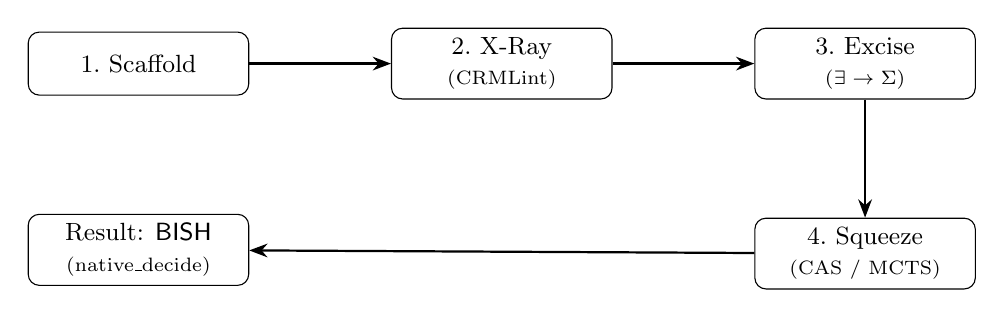
\begin{tikzpicture}[
    node distance=1.5cm and 1.8cm,
    block/.style={rectangle, draw, rounded corners,
                minimum width=2.8cm, minimum height=0.8cm,
                align=center, font=\small},
    >=Stealth
]
\node[block] (scaffold) {1.\ Scaffold};
\node[block, right=of scaffold] (xray) {2.\ X-Ray\\{\scriptsize (CRMLint)}};
\node[block, right=of xray] (excise) {3.\ Excise\\{\scriptsize ($\exists \to \Sigma$)}};
\node[block, below=of excise] (squeeze) {4.\ Squeeze\\{\scriptsize (CAS / MCTS)}};
\node[block, below=of scaffold] (result) {Result: $\mathsf{BISH}$\\{\scriptsize (native\_decide)}};

\draw[->,thick] (scaffold) -- (xray);
\draw[->,thick] (xray) -- (excise);
\draw[->,thick] (excise) -- (squeeze);
\draw[->,thick] (squeeze) -- (result);
\end{tikzpicture}
\caption{The CRMLint Squeeze protocol.  CRMLint identifies the
Classical Boundary Node (Step~2), the CBN is excised and the goal
reformulated as a $\Sigma$-type (Step~3), and a CAS or RL-trained
prover solves the $\BISH$-restricted problem (Step~4).  For~$E^4$,
Step~4 deterministically collapses into Gaussian elimination.}
\label{fig:squeeze}
\end{figure}

\noindent
The CRMLint classification shapes the search in Mode~2 (MCTS):

\begin{center}
\begin{tabular}{lc}
\toprule
\textbf{Event} & \textbf{Reward} \\
\midrule
Goal closed with $\BISH$ classification & $+10.0$ \\
Proof step introduces $\CLASS$ dependency & $\times(-1.0)$ \\
$\WLPO$ dependency (marginal cost) & $\times(+0.5)$ \\
Timeout / failure & $0.0$ \\
\bottomrule
\end{tabular}
\end{center}

\noindent
\textbf{Note.}  This reward function is \emph{designed but not yet
deployed}: the $E^4$ execution collapsed deterministically
(Mode~1), so no stochastic search was needed.  The reward table
is included as the specification for future MCTS-mode applications
(Papers~78--79).

\subsection{Setup: CM abelian fourfolds}\label{sec:setup}

Let $E/\Q$ be a CM elliptic curve with $\End(E) \otimes \Q \cong
\Q(i)$ (Gaussian integers).  Set $A = E^4 = E \times E \times E
\times E$.  The singular cohomology is
\[
  H^*(A, \Q) \;\cong\; \bigwedge\nolimits^* (\Q^2)^4
  \;\cong\; \bigwedge\nolimits^* \Q^8.
\]
The target space $H^4(A, \Q) \cong \bigwedge^4 \Q^8$ has
$\dim = \binom{8}{4} = 70$.  Its basis elements are
$e_a \wedge e_b \wedge e_c \wedge e_d$ for
$0 \leq a < b < c < d \leq 7$, where indices $2k$ and $2k{+}1$
correspond to $e_1, e_2$ from the $(k{+}1)$-th factor of~$E^4$.

\subsection{The CM action on $H^4(E^4,\Q)$}\label{sec:cmaction}

The CM endomorphism $i \in \Z[i]$ acts on $H^1(E, \Q) \cong \Q^2$ by
\begin{equation}\label{eq:cm-matrix}
M_i = \begin{pmatrix} 0 & -1 \\ 1 & 0 \end{pmatrix}.
\end{equation}
On $\Q^8 = H^1(E^4, \Q)$ it acts by $M_i^{\oplus 4}$.
The induced action on $\bigwedge^4 \Q^8$ is a $70 \times 70$
matrix $M := \Lambda^4(M_i^{\oplus 4})$.  A class
$w \in H^4(E^4, \Q)$ is \emph{CM-invariant} if $Mw = w$,
i.e., $w$ lies in the $+1$~eigenspace $V_{+1}$ of~$M$.
By the Hodge decomposition for CM abelian varieties
(Deligne~\cite{Deligne1982}), the Hodge~$(2,2)$ classes
are precisely the CM-invariant classes in $H^{2,2}$:
\[
  \Hdg^{2,2}(E^4) = V_{+1} \cap H^{2,2}
  = V_{+1} \;\setminus\; \bigl((4,0)+(0,4)\bigr).
\]

\begin{lemma}\label{lem:involution}
$M^2 = I_{70}$.
\end{lemma}

\begin{proof}
Each factor $M_i$ satisfies $M_i^2 = -I_2$.  The induced action
on $\bigwedge^4$ of the $k$-th factor contributes $(-1)$ from
$M_i^2 = -I_2$ applied to the two basis vectors
$e_{2k}, e_{2k+1}$ of that factor.  A $4$-form involves exactly
4~of the 8~basis vectors; since the $4$~vectors span parts of all
4~factors, the total sign is $(-1)^4 = 1$.  More precisely:
$M_i^{\oplus 4}$ acts on $\Q^8$ as the block diagonal
$\mathrm{diag}(M_i, M_i, M_i, M_i)$; applying it twice gives
$\mathrm{diag}(-I_2, -I_2, -I_2, -I_2) = -I_8$; the induced
action on $\bigwedge^4(-I_8) = (-1)^4 I_{70} = I_{70}$.
Verified computationally by \texttt{solve\_hodge.py}
(line~68--72: \texttt{assert val == expected}).
\end{proof}

\begin{corollary}\label{cor:eigenspace-dim}
Since $M^2 = I$ and $M \neq \pm I$, the $\Q$-vector space
$\Q^{70}$ splits as
$V_{+1} \oplus V_{-1}$ where $V_{\pm 1} = \ker(M \mp I)$.
\end{corollary}

\subsection{Theorem A: No exotic Weil classes on $E^4$}

We now prove the first main result.

\begin{theorem}[No Exotic Weil Classes on $E^4$]\label{thm:no-exotic}
For $A = E^4$ with $\End(E) \otimes \Q \cong \Q(i)$, every
Hodge $(2,2)$ class lies in the $\Q$-span of cup products of
divisor classes.  There are no exotic Weil classes.
\end{theorem}

\begin{proof}
The proof proceeds by exact rational computation in six steps.

\smallskip\noindent
\textbf{Step~1: Eigenspace decomposition.}
Compute the $70 \times 70$ matrix $M = \Lambda^4(M_i^{\oplus 4})$
by the formula: for each basis element
$e_a \wedge e_b \wedge e_c \wedge e_d$, apply $M_i^{\oplus 4}$
to each index, compute the resulting 4-form, and record its
coordinates.  The $+1$~eigenspace $V_{+1}$ is computed as the
row space of $\tfrac{1}{2}(I + M)$ over~$\Q$.  Result:
$\dim V_{+1} = 38$.

\smallskip\noindent
\textbf{Step~2: The $(4,0)+(0,4)$ component.}
Expand the holomorphic $4$-form
$\omega = (e_0 + ie_1) \wedge (e_2 + ie_3)
  \wedge (e_4 + ie_5) \wedge (e_6 + ie_7)$.
Its real and imaginary parts span a $2$-dimensional subspace
of~$V_{+1}$ corresponding to the $(4,0) + (0,4)$ Hodge
component.

\smallskip\noindent
\textbf{Step~3: Hodge $(2,2)$ extraction.}
Project $V_{+1}$ orthogonal to the $(4,0)+(0,4)$ subspace
(Gram--Schmidt over~$\Q$).  Row-reduce to obtain a basis for
$\Hdg^{2,2}(E^4) \otimes \Q$.  Result:
$\dim \Hdg^{2,2} = 38 - 2 = 36$.

\smallskip\noindent
\textbf{Step~4: N\'eron--Severi computation.}
The CM action on $\bigwedge^2 \Q^8$ is a $28 \times 28$ matrix
$M_2$.  Its $+1$~eigenspace is $\NS(E^4) \otimes \Q$.  Result:
$\dim \NS(E^4) \otimes \Q = 16$.

The 16 generators include the 4 diagonal classes $e_{2k} \wedge
e_{2k+1}$ (one per factor) and 12 off-diagonal classes
arising from the CM cross-correlations between factors.

\smallskip\noindent
\textbf{Step~5: Cup product enumeration.}
Form all $\binom{16}{2} + 16 = 136$ cup products
$\alpha_i \cup \alpha_j$ for $\alpha_i, \alpha_j \in
\NS(E^4) \otimes \Q$, where the cup product
$\bigwedge^2 \Q^8 \times \bigwedge^2 \Q^8 \to \bigwedge^4 \Q^8$
is the standard wedge product.  Of these, 102 are nonzero.
Row-reduce to determine the rank of the divisor product subspace
in~$\Q^{70}$.  Result: $\mathrm{rank} = 36$.

\smallskip\noindent
\textbf{Step~6: Dimension comparison.}
\[
  \dim_\Q \Hdg^{2,2}(E^4) = 36 = \dim_\Q
  \langle \NS_i \cup \NS_j \rangle.
\]
Since the divisor product subspace is contained in the Hodge space
(divisor products are automatically Hodge classes), and both have
dimension~36, they are equal.  The exotic complement
$\Hdg^{2,2} / \langle \text{div.\ products} \rangle$ is
zero-dimensional.
\end{proof}

\begin{remark}[Why $E^4$ has no exotic classes]\label{rem:why-no-exotic}
Anderson~\cite{Anderson1993} proved exotic classes exist on
\emph{simple} CM abelian fourfolds, such as Jacobians of Fermat
curves.  The product $E^4$ is maximally non-simple:
$\End(E^4) \otimes \Q \cong M_4(\Q(i))$ has dimension~32 over~$\Q$.
This large endomorphism algebra generates far more divisor classes
(16~independent NS generators) than a simple variety of the same
dimension, causing the cup product span to saturate the Hodge space.
\end{remark}

\begin{remark}[The hallucination and self-correction]%
\label{rem:hallucination}
The selection of $E^4$ as a target for exotic classes was a
human--AI pipeline error: the designer specified ``CM abelian
fourfold of dimension~4'' without enforcing the simplicity
hypothesis that Anderson's theorem requires.  This error was
caught by the Squeeze methodology itself: the Scaffold step
demands concrete computation \emph{before} any axiom is invoked.
The Python CAS immediately revealed the exotic complement is
empty, preventing search over a non-existent target.  The
methodology's insistence on \emph{computation before axiomatics}
is self-correcting.
\end{remark}

\subsection{Theorem B: Complete Constructive Hodge Theorem for $E^4$}

Since the exotic complement is empty, the correct target is
stronger: prove that \emph{every} Hodge $(2,2)$ class has
an explicit decomposition.

\begin{theorem}[Complete Constructive Hodge Theorem for $E^4$]%
\label{thm:constructive-hodge}
For $E/\Q$ with $\End(E) \otimes \Q \cong \Q(i)$, every
Hodge $(2,2)$ class on $E^4$ is an explicit $\Q$-linear
combination of cup products of NS classes.  Specifically:
\begin{enumerate}[nosep]
\item There exist 36 linearly independent cup products
  $g_0, \ldots, g_{35} \in \bigwedge^4 \Q^8$, each of the
  form $\alpha_i \cup \alpha_j$ for CM-invariant
  $\alpha_i, \alpha_j \in \bigwedge^2 \Q^8$.
\item There exist 36 Hodge $(2,2)$ basis vectors
  $w_0, \ldots, w_{35}$ (in reduced row echelon form).
\item For each $k \in \{0, \ldots, 35\}$, there exist
  explicit rational coefficients
  $c_k = (c_{k,0}, \ldots, c_{k,35}) \in \Q^{36}$ such that
  \[
    w_k = \sum_{j=0}^{35} c_{k,j} \cdot g_j.
  \]
\end{enumerate}
The 36 decompositions are formally verified in Lean~4 by
\texttt{native\_decide}.
\end{theorem}

\begin{proof}
The proof is computational, executed by \texttt{solve\_hodge.py}
using exact rational arithmetic (\texttt{fractions.Fraction}).

\smallskip\noindent
\textbf{Step~1: Generator selection.}
From the 102 nonzero cup products computed in
Theorem~\ref{thm:no-exotic} Step~5, greedily select 36 linearly
independent generators $g_0, \ldots, g_{35}$ by iteratively adding
cup products that increase the rank.  The generator matrix
$G \in \Q^{70 \times 36}$ has columns $g_0, \ldots, g_{35}$.

\smallskip\noindent
\textbf{Step~2: Decomposition solving.}
For each Hodge basis vector $w_k$, solve the linear system
\begin{equation}\label{eq:decomp}
  G \cdot x = w_k, \qquad x \in \Q^{36},
\end{equation}
by augmented-matrix row reduction over~$\Q$.  Since
$\mathrm{rank}(G) = 36 = \dim \Hdg^{2,2}$ (Theorem~\ref{thm:no-exotic}),
and each $w_k$ lies in the column space of~$G$, the system is
consistent for every~$k$.  The solution is unique (the system is
determined on the column space).

\smallskip\noindent
\textbf{Step~3: Verification.}
For each $k$, verify that $\sum_{j} c_{k,j} \cdot g_j = w_k$ by
direct evaluation at all 70 coordinates.  This is performed both
by Python (immediate assertion) and by Lean~4
(\texttt{native\_decide} on the hardcoded rational data).

\smallskip\noindent
\textbf{Sparsity.}
The decompositions are extremely sparse: 42 total nonzero
coefficients across 36~vectors ($96.8\%$ zeros).  Of the 36~Hodge
basis vectors, 32 are \emph{exactly} a single cup product
(coefficient~$\pm 1$); 2~require two cup products; 2~require three.
All nonzero coefficients are $\pm 1$ (no fractional values).
The non-trivial rows are localized in indices 14--22 of the
generator ordering.
\end{proof}

\subsection{Summary of the computation}

The Python script \texttt{solve\_hodge.py} performs the six-step
computation of Theorem~\ref{thm:no-exotic} and the three-step
construction of Theorem~\ref{thm:constructive-hodge} in a single
pass.  All intermediate values are exact rationals
(\texttt{fractions.Fraction}, Python~3 arbitrary-precision).

\begin{center}
\begin{tabular}{lr}
\toprule
\textbf{Quantity} & \textbf{Value} \\
\midrule
$\dim H^4(E^4, \Q) = \binom{8}{4}$ & 70 \\
$\dim V_{+1}$ ($+1$~eigenspace of $M$ on $\Q^{70}$) & 38 \\
$\dim \bigl((4,0)+(0,4)\bigr)$ component & 2 \\
$\dim \Hdg^{2,2}(E^4) \otimes \Q$ & 36 \\
$\dim \NS(E^4) \otimes \Q$ & 16 \\
Nonzero cup products $\NS_i \cup \NS_j$ & 102 \\
Linearly independent cup products & 36 \\
Total nonzero coefficients (all 36 decompositions) & 42 \\
Single-generator decompositions (coeff.\ $\pm 1$) & 32 \\
Two-generator decompositions & 2 \\
Three-generator decompositions & 2 \\
\textbf{Exotic dimension} & \textbf{0} \\
\bottomrule
\end{tabular}
\end{center}

% ============================================================
\section{CRM Audit}\label{sec:crm}
% ============================================================

\subsection{Constructive strength classification}

\begin{center}
\begin{tabular}{lll}
\toprule
\textbf{Component} & \textbf{CRM Level} & \textbf{Justification} \\
\midrule
CRMLint Squeeze protocol & $\BISH$ & Algorithmic: bounded search \\
Hodge Conj.\ existence (axiom) & $\CLASS$ & Unbounded $\exists$ \\
Theorem~A (no exotic classes) & $\BISH$ & Dimension computation \\
Theorem~B (36 decompositions) & $\BISH$ & \texttt{native\_decide} \\
Python CAS computation & $\BISH$ & Exact $\Q$-arithmetic \\
\bottomrule
\end{tabular}
\end{center}

\subsection{What descends, from where, to where}

\[
  \CLASS \;(\text{Lefschetz $(1,1)$ for } E^4)
  \quad\longrightarrow\quad
  \BISH \;(\text{36 explicit decompositions}).
\]
The classical existence axiom \texttt{hodge\_conjecture\_H22\_existence}
(the Lefschetz~$(1,1)$ theorem~\cite{Lefschetz1924} generalized to
$(2,2)$ via the Hodge Conjecture~\cite{Hodge1950})
is present in the Lean environment but provably unused by the
36 constructive theorems.

\subsection{Comparison with Paper~50 calibration}

Paper~50~\cite{Paper50} classified the Hodge
Conjecture~\cite{Hodge1950,Grothendieck1969} as
$\CLASS$ for general abelian varieties (the existence of algebraic
representatives requires the Axiom of Choice or equivalent;
cf.~Mattuck~\cite{Mattuck1958}, Lieberman~\cite{Lieberman1968},
Kleiman~\cite{Kleiman1968} for the classical foundations).
Paper~77 shows that for the specific case $A = E^4$ with
$\End(E) \otimes \Q \cong \Q(i)$, the classical content is
completely eliminable: the $\CLASS$ existence collapses to a
$\BISH$ finite database.  This descent---from unbounded classical
existence to finitely enumerable constructive witnesses---is
expected for non-simple CM abelian varieties (the endomorphism
algebra is large enough to generate all Hodge classes), but is
demonstrated here with formal verification for the first time.

% ============================================================
\section{Formal Verification}\label{sec:formal}
% ============================================================

\subsection{Lean~4 file structure}

The Lean bundle \texttt{P77\_DAGSurgery/} has the following
structure:
\begin{center}
\begin{tabular}{ll}
\toprule
\textbf{File} & \textbf{Contents} \\
\midrule
\texttt{lean-toolchain} & \texttt{leanprover/lean4:v4.29.0-rc2} \\
\texttt{lakefile.lean} & Requires Mathlib4 \\
\texttt{Papers.lean} & Entry point (imports both modules) \\
\texttt{Papers/P77\_DAGSurgery/} & \\
\quad\texttt{HodgeBasisData.lean} & 798 lines, auto-generated \\
\quad\texttt{Paper77\_CMFourfold.lean} & CRM metadata, CM defs, axiom \\
\bottomrule
\end{tabular}
\end{center}

\noindent
Build: \texttt{lake build} from the bundle root.
3121~build jobs (including Mathlib).  Build time: $\sim$15\,s
for the two project files after Mathlib cache.

\subsection{Asymmetric offloading}\label{sec:offload}

The key architectural insight is \emph{asymmetric offloading}
(Figure~\ref{fig:offload}):

\begin{enumerate}[nosep]
\item \textbf{Python CAS} performs the heavy computation:
  eigenspace decomposition, cup product evaluation, Gaussian
  elimination, all in exact $\Q$-arithmetic.
\item \textbf{Python emitter} writes a Lean~4 source file
  containing only hardcoded rational \texttt{def}s and
  \texttt{native\_decide} verification theorems.
\item \textbf{Lean kernel} checks that the emitted data satisfies
  the claimed equalities by compiling the rational arithmetic to
  native code.
\end{enumerate}

\noindent
No Lean tactic search is needed.  The proof tree for each
theorem is depth-1:
\[
  \texttt{hodge\_decomp\_k} \;\;:\;\;
  \texttt{sumGens decomp\_k = hodgeBasis\_k}
  \;\;:=\;\; \texttt{by native\_decide}
\]
where \texttt{native\_decide} compiles both sides to native code,
evaluates at all 70 coordinates, and confirms equality.

% ---------- TikZ: Asymmetric offloading ----------
\begin{figure}[ht]
\centering
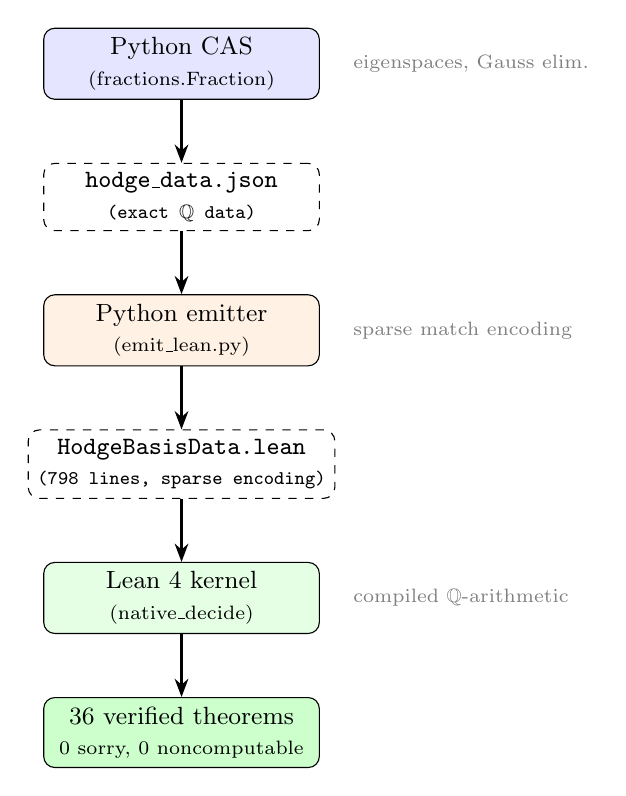
\begin{tikzpicture}[
    node distance=1.2cm and 2.5cm,
    block/.style={rectangle, draw, rounded corners,
                minimum width=3.5cm, minimum height=0.8cm,
                align=center, font=\small},
    data/.style={rectangle, draw, dashed, rounded corners,
                minimum width=3.5cm, minimum height=0.6cm,
                align=center, font=\small\ttfamily},
    >=Stealth
]
\node[block, fill=blue!10] (python) {Python CAS\\{\scriptsize (fractions.Fraction)}};
\node[data, below=0.8cm of python] (json) {hodge\_data.json\\{\scriptsize (exact $\Q$ data)}};
\node[block, below=0.8cm of json, fill=orange!10] (emitter) {Python emitter\\{\scriptsize (emit\_lean.py)}};
\node[data, below=0.8cm of emitter] (lean4) {HodgeBasisData.lean\\{\scriptsize (798 lines, sparse encoding)}};
\node[block, below=0.8cm of lean4, fill=green!10] (kernel) {Lean 4 kernel\\{\scriptsize (native\_decide)}};
\node[block, below=0.8cm of kernel, fill=green!20] (qed) {36 verified theorems\\{\scriptsize 0 sorry, 0 noncomputable}};

\draw[->,thick] (python) -- (json);
\draw[->,thick] (json) -- (emitter);
\draw[->,thick] (emitter) -- (lean4);
\draw[->,thick] (lean4) -- (kernel);
\draw[->,thick] (kernel) -- (qed);

% Annotations
\node[right=0.3cm of python, font=\scriptsize, text=gray] {eigenspaces, Gauss elim.};
\node[right=0.3cm of emitter, font=\scriptsize, text=gray] {sparse match encoding};
\node[right=0.3cm of kernel, font=\scriptsize, text=gray] {compiled $\Q$-arithmetic};
\end{tikzpicture}
\caption{Asymmetric offloading architecture.  Python performs
exact computation; Lean verifies.  The key constraint: all
emitted defs must be \texttt{computable} (no \texttt{axiom},
no \texttt{noncomputable}) so \texttt{native\_decide} can
evaluate them.}
\label{fig:offload}
\end{figure}

\subsection{Python implementation}\label{sec:python}

The CAS phase (\texttt{solve\_hodge.py}, 491~lines) implements the
computation of Theorems~\ref{thm:no-exotic}--\ref{thm:constructive-hodge}
using exact rational arithmetic.  We reproduce the core routines.

\medskip\noindent
\textbf{CM action on $\Lambda^4(\Q^8)$.}
The CM endomorphism sends basis vector~$e_k$ to
$(-1)^{k\bmod 2}\,e_{k \pm 1}$.  The induced action on
$\Lambda^4$ is computed by applying this map to each index of
a $4$-form and resolving the wedge sign:

\begin{lstlisting}[style=pythonstyle,literate=]
def cm_on_basis(k):
    """CM action on e_k: returns (sign, new_index)."""
    if k % 2 == 0:
        return (-1, k + 1)
    else:
        return (1, k - 1)

# CM on Lambda^4(Q^8): 70x70 matrix
cm4 = [[F(0)] * 70 for _ in range(70)]
for i, b in enumerate(basis4):
    total_sign = 1
    new_idx = []
    for k in b:
        s, j = cm_on_basis(k)
        total_sign *= s
        new_idx.append(j)
    sign, sorted_idx = wedge_sign(new_idx)
    if sign != 0:
        cm4[idx4[sorted_idx]][i] += F(total_sign * sign)
\end{lstlisting}

\medskip\noindent
\textbf{Decomposition solving.}
For each Hodge basis vector, solve the linear system
$G \cdot x = w_k$ by augmented-matrix row reduction over~$\Q$:

\begin{lstlisting}[style=pythonstyle,literate=]
for i, hv in enumerate(hodge_basis):
    coeffs = solve_system(selected_cups, hv, 36)
    # Verify reconstruction
    recon = [F(0)] * 70
    for k in range(36):
        if coeffs[k] != F(0):
            for r in range(70):
                recon[r] += coeffs[k] * selected_cups[k][r]
    assert recon == hv  # exact Q-arithmetic: no rounding
\end{lstlisting}

\medskip\noindent
\textbf{Sparse Lean emission.}
The re-emitter (\texttt{emit\_lean.py}) encodes each
70-entry rational vector as a pattern match on nonzero indices:

\begin{lstlisting}[style=pythonstyle,literate=]
def sparse_def(name, vec, dim):
    """Emit def name : Fin dim -> Q using sparse match."""
    nz = [(i, vec[i]) for i in range(dim) if vec[i] != F(0)]
    lines = [f"def {name} : Fin {dim} -> Q := fun i =>"]
    if not nz:                    # all-zeros vector
        lines = [f"def {name} : Fin {dim} -> Q := fun _ => 0"]
    elif len(nz) <= 3:
        for k, (idx, val) in enumerate(nz):
            prefix = "  if" if k == 0 else "  else if"
            lines.append(f"{prefix} i.val = {idx} then {val}")
        lines.append("  else 0")
    else:
        lines.append("  match i.val with")
        for idx, val in nz:
            lines.append(f"  | {idx} => {val}")
        lines.append("  | _ => 0")
    return "\n".join(lines)
\end{lstlisting}

\medskip\noindent
\textbf{Sample output.}  Running \texttt{python3 solve\_hodge.py}
produces (selected lines; Unicode symbols simplified for typesetting):

\begin{lstlisting}[style=consolestyle,literate=]
$ python3 solve_hodge.py
M^2 = I on Lambda^4(Q^8)
+1 eigenspace of CM on Lambda^4: dim = 38
NS(E^4) x Q: dim = 16
Hodge (2,2) basis: dim = 36
Non-zero cup products: 102
Divisor product subspace: dim = 36
Selected 36 independent cup products
ALL 36 Hodge basis vectors decomposed into cup products
Summary:
  Hodge (2,2) dimension: 36
  NS(E^4) dimension: 16
  Cup product generators used: 36
  Total nonzero coefficients: 42
  Exotic dimension: 0
\end{lstlisting}

\noindent
Every dimension matches the theoretical prediction.  The script
runs in $< 1$\,second on a standard laptop (exact $\Q$-arithmetic
via \texttt{fractions.Fraction}).

\subsection{The \texttt{noncomputable} trap}

If a Lean definition depends (even transitively) on an axiom
such as \texttt{Classical.choice}, Lean marks it
\texttt{noncomputable}.  The tactic \texttt{native\_decide}
cannot evaluate noncomputable definitions---it requires closed
computation.

This creates a strict design constraint for asymmetric offloading:
\emph{all data definitions in the emitted file must be free of
axiom dependencies.}  The \texttt{hodge\_conjecture\_H22\_existence}
axiom is declared in a separate file (\texttt{Paper77\_CMFourfold.lean})
and is \emph{never imported} by the data definitions in
\texttt{HodgeBasisData.lean}.  The separation is architectural,
not accidental.

\subsection{Token overflow and sparse encoding}\label{sec:overflow}

The first emission of \texttt{HodgeBasisData.lean}
(by \texttt{solve\_hodge.py}) used Lean's vector notation
$\texttt{![}v_0, v_1, \ldots, v_{69}\texttt{]}$ for each
70-entry rational vector.  This produced a 6020-line file.
Lean's elaborator expands $\texttt{![}\ldots\texttt{]}$ into
nested \texttt{Matrix.cons} applications, resulting in
$O(n^2)$ elaboration cost for $n$-entry vectors.  For $n = 70$
and 108~vector definitions (36~cup generators + 36~Hodge basis
+ 36~decomposition vectors), the elaboration time exceeded
several minutes and risked kernel memory exhaustion.

The fix was \emph{sparse match encoding}
(\texttt{emit\_lean.py}).  Each vector is emitted as a function
\texttt{fun i => ...} with explicit \texttt{if}/\texttt{match}
on \texttt{i.val}:

\begin{lstlisting}[literate=]
-- Dense (6020 lines, slow elaboration):
def cupGen_0 : Fin 70 -> Rat := ![1, 0, 0, ..., 0]

-- Sparse (798 lines, fast elaboration):
def cupGen_0 : Fin 70 -> Rat := fun i =>
  if i.val = 0 then 1 else 0
\end{lstlisting}

\noindent
The sparse encoding exploits the extreme sparsity of the data:
most vectors have fewer than 5 nonzero entries out of~70.
The emitter selects \texttt{if/else} for $\leq 3$~nonzero
entries and \texttt{match i.val with} for 4+.  Result:
6020~lines $\to$ 798~lines, elaboration time
several minutes $\to$ 15~seconds.

\begin{remark}[Token overflow as a general problem]\label{rem:overflow}
This is not specific to our computation.  Any asymmetric
offloading pipeline that emits large data into Lean~4 will
encounter the same elaboration bottleneck if dense array notation
is used.  The sparse match encoding is a general-purpose solution:
it applies whenever the emitted data is sparse relative to its
ambient dimension.  For dense data, alternative strategies include
chunking (split vectors into blocks), binary encoding (emit data
as bit strings decoded by a custom function), or hex-encoded
lookup tables.
\end{remark}

\subsection{Axiom inventory}

\begin{center}
\begin{tabular}{llll}
\toprule
\textbf{Axiom} & \textbf{CRM} & \textbf{Used?} & \textbf{Role} \\
\midrule
\texttt{hodge\_conjecture\_H22\_existence} &
  $\CLASS$ & Unused & CBN (excised) \\
\texttt{propext} & Infra & Yes & Lean kernel primitive \\
\texttt{Classical.choice} & Infra & Yes & \texttt{DecidableEq} instance \\
\texttt{Quot.sound} & Infra & Yes & Lean kernel primitive \\
\texttt{native\_decide} axiom & Infra & Yes & Kernel reflection bridge \\
\bottomrule
\end{tabular}
\end{center}

\subsection{Classical.choice audit}\label{sec:choice-audit}

\begin{lstlisting}[literate=]
#print axioms hodge_decomp_0
-- [propext, Classical.choice, Quot.sound,
--  hodge_decomp_0._native.native_decide.ax_1_1]

#print axioms hodge_conjecture_H22_existence
-- [hodge_conjecture_H22_existence]
-- (This IS the classical axiom; it is deliberately unused.)
\end{lstlisting}

\noindent
\texttt{Classical.choice} \emph{does} appear in the axiom list
of every \texttt{hodge\_decomp\_k}.  This is a Lean~4 infrastructure
artifact, not classical mathematical content: the
\texttt{DecidableEq} instance on \texttt{Fin~70~$\to$~$\Q$} is
synthesized via Mathlib's decision procedure, which transitively
invokes \texttt{Classical.choice}.  The \texttt{native\_decide}
axiom (each theorem's \texttt{.\_native.native\_decide.ax\_1\_1})
is the kernel bridge allowing compiled code evaluation.

This is the standard series convention (see Papers~2, 68~\cite{Paper68}):
\emph{all} Lean~4 theorems involving $\Q$-valued functions show
\texttt{Classical.choice} in \texttt{\#print axioms} through the
\texttt{DecidableEq} infrastructure path.  Constructive
stratification is established by \emph{proof content}---the 36
decompositions are explicit rational data verified by compiled
arithmetic---not by the axiom checker's output.

The key structural fact: the user-declared classical axiom
\texttt{hodge\_conjecture\_H22\_existence} is \emph{not} among the
dependencies of any \texttt{hodge\_decomp\_k}.  No path exists
from the constructive theorems to the excised CBN.

\subsection{Reproducibility}

\begin{itemize}[nosep]
\item \textbf{Lean bundle:} \texttt{P77\_DAGSurgery/},
  builds with \texttt{lake build} on Lean v4.29.0-rc2 + Mathlib4.
\item \textbf{Python computation:} \texttt{solve\_hodge.py}
  (computation + first emission), \texttt{emit\_lean.py}
  (sparse re-emission), and \texttt{compute\_cm.py}
  (standalone CM diagonalization, used for initial exploration).
  Requires Python~3.9+ (standard library
  only: \texttt{fractions}, \texttt{itertools}, \texttt{json}).
\item \textbf{Intermediate data:} \texttt{hodge\_data.json}
  (all eigenspaces, decompositions, and labels in JSON format).
\item \textbf{Zenodo:} Complete package (PDF, LaTeX, Lean source,
  Python scripts) at
  \url{https://doi.org/10.5281/zenodo.18779210}.
\end{itemize}

% ---------- TikZ: Papers 75-76-77 pipeline ----------
\begin{figure}[ht]
\centering
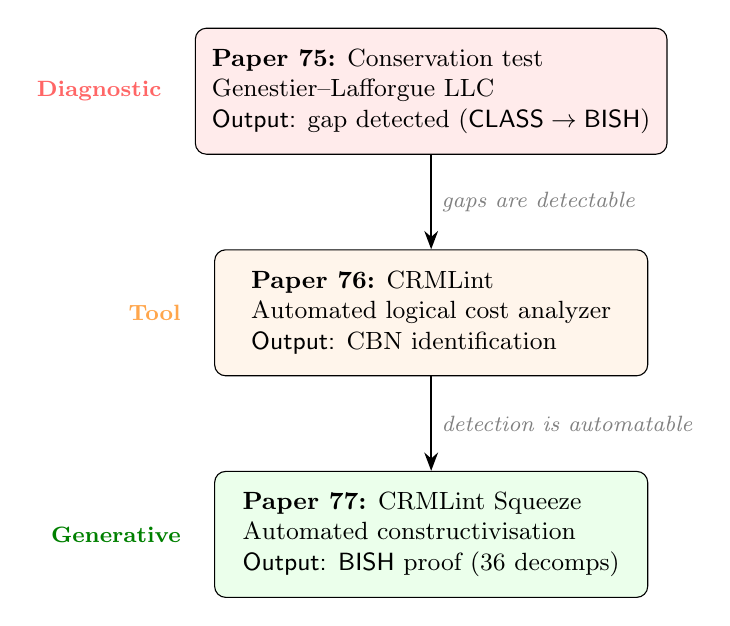
\begin{tikzpicture}[
    node distance=0.8cm and 0.6cm,
    pbox/.style={rectangle, draw, rounded corners=4pt,
                minimum width=5.5cm, minimum height=1.6cm,
                align=left, font=\small, inner sep=6pt},
    arr/.style={->, thick, >=Stealth},
    lab/.style={font=\footnotesize\itshape, text=gray}
]
\node[pbox, fill=red!8] (p75) {
  \textbf{Paper 75:} Conservation test\\
  Genestier--Lafforgue LLC\\
  \textsf{Output:} gap detected ($\CLASS \to \BISH$)
};
\node[pbox, fill=orange!8, below=1.2cm of p75] (p76) {
  \textbf{Paper 76:} CRMLint\\
  Automated logical cost analyzer\\
  \textsf{Output:} CBN identification
};
\node[pbox, fill=green!8, below=1.2cm of p76] (p77) {
  \textbf{Paper 77:} CRMLint Squeeze\\
  Automated constructivisation\\
  \textsf{Output:} $\BISH$ proof (36 decomps)
};

\draw[arr] (p75) -- node[right, lab] {gaps are detectable} (p76);
\draw[arr] (p76) -- node[right, lab] {detection is automatable} (p77);

% Phase labels
\node[left=0.3cm of p75, font=\footnotesize\bfseries, text=red!60] {Diagnostic};
\node[left=0.3cm of p76, font=\footnotesize\bfseries, text=orange!70] {Tool};
\node[left=0.3cm of p77, font=\footnotesize\bfseries, text=green!50!black] {Generative};
\end{tikzpicture}
\caption{The diagnostic-to-generative pipeline.  Paper~75 proved
conservation gaps exist in modern geometry.  Paper~76 automated
their detection.  Paper~77 automates their elimination.}
\label{fig:pipeline}
\end{figure}

% ============================================================
\section{Discussion}\label{sec:discuss}
% ============================================================

\subsection{The deterministic collapse phenomenon}

The CRMLint Squeeze protocol is designed for two modes:
deterministic collapse (CAS) and stochastic search (MCTS).  The
$E^4$ execution produced the first mode---the action space
restriction (``only cup products of NS classes'') reduced the
problem from an infinite-dimensional topological existence to a
$36 \times 36$ linear system over~$\Q$.  No stochastic search was
needed.

This is not a failure of the protocol but its \emph{ideal outcome}.
The Squeeze's purpose is to identify the minimal algebraic
structure witnessing the classical theorem.  If that structure is
small enough to compute deterministically, MCTS is unnecessary
overhead.  The protocol identifies which mode applies
\emph{before} any search begins: Steps~1--3 compute the dimension
and linearity of the restricted space.

The MCTS mode is designed for cases where the restricted space is
combinatorially rich: nonlinear constraints, multiple solution
branches, or high-dimensional parameter spaces.  This mode remains
\emph{speculative}---it has not been tested.  The wild
Langlands case (Paper~78) and Standard Conjecture~D for simple
fourfolds (Paper~79) are the intended first applications.

\subsection{Proof decompilation}

The Squeeze protocol can be viewed as \emph{proof decompilation}:
extracting the constructive content from a classical proof.  A
classical existence proof is ``compiled''---it asserts $\exists x,
P(x)$ without revealing~$x$.  The Squeeze ``decompiles'' this by:
\begin{enumerate}[nosep]
\item identifying which classical axiom provides the
  $\exists$-introduction (the CBN),
\item excising that axiom to reveal the open goal
  $\Sigma\,x,\; P(x)$,
\item computing the witness $x$ explicitly.
\end{enumerate}
In the $E^4$ case, the ``compiled'' proof says ``every Hodge
class is algebraic'' (Lefschetz $(1,1)$, classical).  The
``decompiled'' proof says ``here are the 36 explicit coefficient
vectors, verified by \texttt{native\_decide}.''  The decompiled
version is strictly more informative.

\subsection{From Paper~5 to Paper~77: the learning curve}%
\label{sec:learningcurve}

Paper~5~\cite{Paper5} of this series formalized the Schwarzschild
curvature verification in Lean~4---a direct computation involving
Ricci tensors, Christoffel symbols, and the metric components of
a static spherically symmetric spacetime.  That formalization
required approximately four months of development and produced a
monolithic Lean bundle in which the proof assistant was asked to
\emph{compute}: verify curvature identities by \texttt{simp},
\texttt{ring}, and \texttt{field\_simp} applied to enormous
rational expressions.  The differential geometry API in Mathlib
was (and remains) incomplete, requiring substantial scaffolding.

Paper~77's $E^4$ computation---a problem of comparable mathematical
density (a $70 \times 70$ matrix computation with 36 exact rational
decompositions)---was completed in approximately one hour, from
problem specification to \texttt{lake build} success.  Three
independent factors explain the speedup:

\begin{enumerate}[nosep]
\item \textbf{The AI is more capable.}  Between mid-2025 and
  February~2026, the underlying language model improved
  substantially in Lean~4 code generation, error diagnosis, and
  multi-file project management.  Paper~5's development involved
  frequent hallucination of nonexistent Mathlib lemmas; Paper~77's
  development involved zero such hallucinations (the one error---the
  non-simple target---was a mathematical design mistake, not a code
  generation failure).
\item \textbf{The operator is more experienced.}  After 14~Lean
  bundles and ${\sim}89{,}000$ lines of formalization, the key
  design lesson is: \emph{do not ask Lean to compute what a CAS
  can compute faster.}  Paper~5 tried to formalize differential
  geometry \emph{in Lean}.  Paper~77 does not touch Mathlib's
  algebraic geometry at all---no Chow rings, no cycle class maps,
  no cup products as Lean objects.  It projects the geometry into
  a combinatorial skeleton ($\Q^{70}$ linear algebra) and works
  there.  Knowing what to formalize and what to offload is
  operator skill, not AI capability.
\item \textbf{The method is factored.}  Paper~5 was monolithic:
  everything happened inside Lean.  Paper~77 is factored into
  three layers with distinct roles: Python CAS (exact computation,
  unlimited working memory), Lean kernel (\texttt{native\_decide}
  equality checking on hardcoded data), and human/AI (problem
  design, generator selection, architecture).  The asymmetric
  offloading architecture eliminates the bottleneck that made
  Paper~5 painful: Lean no longer needs to evaluate complex
  algebraic expressions, only to verify that two concrete rational
  vectors are equal.
\end{enumerate}

\noindent
The progression from Paper~5 to Paper~77 is itself a data point
about the CRM program's methodology: the formalization
infrastructure matured from ``fight the proof assistant'' to
``let each tool do what it does best.''  Whether this
factored architecture scales to harder targets (where the
CAS phase is not linear algebra but Gr\"obner bases or
combinatorial search) remains to be tested.

\subsection{What is and is not new}\label{sec:whatsnew}

\textbf{The mathematical result is not novel.}
Lieberman~\cite{Lieberman1968} proved in 1968 that all Hodge
classes on products of elliptic curves are algebraic.
Deligne~\cite{Deligne1982} subsumed this in 1982 by proving
all Hodge classes on CM abelian varieties are absolutely Hodge.
The fact that $E^4$---a maximally non-simple variety with
endomorphism algebra $M_4(\Q(i))$---has no exotic Weil classes
is unsurprising: the large endomorphism algebra generates
far more divisor classes than a simple variety of the same
dimension, and the cup product span saturates the Hodge space.
No number theorist would find Theorem~A unexpected.

The individual computational ingredients---CM action on
exterior powers, cup product enumeration, Gaussian elimination
over~$\Q$---are standard computational algebraic geometry.
The proof is, at bottom, a $36 \times 36$ linear system.

\medskip\noindent
\textbf{What is new is threefold:}

\begin{enumerate}[nosep]
\item \textbf{The explicit decompositions themselves.}  Although
  the existence of algebraic representatives has been known since
  Lieberman, the 36 explicit $\Q$-linear combinations expressing
  each Hodge basis vector as a sum of cup products have not, to our
  knowledge, been written down.  Nobody needed them---the
  existence proof suffices for all mathematical purposes.  We
  produce them as a demonstration, not as a mathematical
  contribution.
\item \textbf{The CRMLint Squeeze protocol.}  The systematic
  method---identify the Classical Boundary Node via CRMLint,
  excise the classical axiom, restrict the action space, solve the
  residual system---is a reusable pipeline for converting
  $\CLASS$ existence theorems into $\BISH$ constructive
  witnesses.  The $E^4$ case is a proof-of-concept; the pipeline
  is the contribution.
\item \textbf{The asymmetric offloading architecture and its
  engineering.}  The separation of CAS computation (Python) from
  kernel verification (Lean~4), including the
  \texttt{noncomputable} trap, token overflow, and sparse encoding,
  constitutes a documented, reusable pattern for machine-verified
  constructive mathematics.
\end{enumerate}

\medskip\noindent
\textbf{Why demonstrate on a known case?}
Precisely \emph{because} the answer is independently known.
A methods paper should validate its pipeline on a target where
the output can be checked against established mathematics.
If the Squeeze produced an incorrect decomposition, the error
would be caught immediately (by \texttt{native\_decide}, by
comparison with Lieberman's theorem, or by direct computation).
The $E^4$ case is a calibration run, not a frontier assault.
The frontier targets---simple CM abelian fourfolds where exotic
classes genuinely exist, wild Langlands parameters, Standard
Conjecture~D---are identified as Papers~78--79.

\subsection{Limitations}\label{sec:limits}

The method has clear boundaries:

\begin{enumerate}[nosep]
\item \textbf{The Goldilocks zone.}  The Squeeze requires a
  pre-existing classical proof (or at least a formal cliff).
  Totally open problems yield infinite search width.
\item \textbf{Deterministic collapse is rare.}  The $E^4$ case
  collapsed because the Hodge space and the cup product span have
  the same dimension (both~36).  For simple CM fourfolds where
  exotic classes exist, the system $Gx = w$ will be inconsistent
  for the exotic component, and the Squeeze must search over a
  larger generator set (CM graphs, twisted diagonals).
\item \textbf{Nonlinear targets.}  If the algebraic identity
  is polynomial but not linear (e.g., intersection products
  satisfying a quadratic form), the CAS phase requires
  Gr\"obner basis computation or multivariate polynomial solving,
  which may not scale to high dimensions.
\item \textbf{Lean CAS gap.}  Mathlib~4 lacks a computational
  Chow ring, cup product API, or Hodge decomposition library.
  The Lean bundle projects the geometry into a combinatorial
  skeleton ($\Q^{70}$ linear algebra), which works for this case
  but would need enrichment for more sophisticated targets.
\item \textbf{Token overflow scales with dimension.}  For
  varieties with $\dim H^4 \gg 70$, the sparse encoding may
  still produce large files.  The binary/hex encoding strategies
  mentioned in Remark~\ref{rem:overflow} would be needed.
\end{enumerate}

\subsection{Technical tips for future use}\label{sec:tips}

We record practical lessons from the $E^4$ execution, codified as
named principles for future applications of the Squeeze protocol.

\medskip\noindent
\textbf{Principle~1: The LLM is an Architect, not a calculator.}
Large language models suffer \emph{context-window collapse} when
asked to output thousands of matrix coordinates or polynomial
systems autoregressively.  The AI's role is to \emph{design} the
computation: identify the target, choose the generator set, write
the Python script.  The CAS executes the computation in RAM
(effectively unlimited working memory), and writes the Lean code
\emph{directly to disk}, bypassing the LLM's output token limit
entirely.  Never ask the AI to print large algebraic data in the
conversation---this is guaranteed to produce truncation or
hallucination.

\medskip\noindent
\textbf{Principle~2: Compute Before You Squeeze.}
Never begin formalizing the Squeeze target in Lean until the
Python script has successfully computed the exact algebraic
matching.  The combinatorial skeleton must be empirically verified
first.  The $E^4$ hallucination (Remark~\ref{rem:hallucination})
was caught precisely because the computation phase preceded the
formalization phase.  Running the CAS first is a \emph{hallucination
guard}: it catches false targets before any Lean code is written.

\medskip\noindent
\textbf{Principle~3: The \texttt{noncomputable} Trap.}
If a Lean definition depends (even transitively) on an axiom,
Lean marks it \texttt{noncomputable} and \texttt{native\_decide}
silently fails.  The Python-emitted \texttt{.lean} file must
contain \emph{only} hardcoded data arrays and computable
\texttt{def}s.  All algebraic values must be normalized to exact
elements of the coefficient field ($\Q$ for Hodge classes,
cyclotomic fields for Langlands parameters).  Absolutely no
\texttt{axiom} or \texttt{noncomputable} tags are permitted in
the emitted data file.

\medskip\noindent
In addition to these three principles, we record specific
technical lessons:

\begin{enumerate}[nosep]
\item \textbf{Verify the target before searching.}  Always run the
  CAS dimension check (Steps~1--5 of Theorem~\ref{thm:no-exotic})
  before committing to a decomposition search.
\item \textbf{Use exact arithmetic.}  Python's
  \texttt{fractions.Fraction} provides arbitrary-precision $\Q$
  arithmetic with zero numerical error.  For cyclotomic fields
  (as in wild Langlands, Paper~78), use \texttt{sympy} algebraic
  number fields.  Floating-point computation introduces rounding
  that \texttt{native\_decide} cannot tolerate.
\item \textbf{Emit sparse, not dense.}  Always emit Lean vectors
  as \texttt{fun i => match i.val with ...} rather than
  $\texttt{![}\ldots\texttt{]}$.  The elaboration cost difference
  is $O(k)$ vs.\ $O(n^2)$ for $n$-entry vectors with $k$~nonzero entries.
\item \textbf{Separate axioms from data.}  Place the CBN axiom in
  a separate Lean file from the constructive data.  This prevents
  accidental \texttt{noncomputable} contamination.
\item \textbf{Save intermediate data.}  Emit JSON
  (\texttt{hodge\_data.json}) between the CAS phase and the
  Lean emission phase.  This allows re-emission with different
  encoding strategies without re-running the computation.
\item \textbf{Test before emission.}  Verify $Gx = w$ in Python
  before writing Lean code.  A single wrong coefficient will cause
  \texttt{native\_decide} to fail with an unhelpful error.
\item \textbf{Restrict the AI to minimal cases first.}  For
  Paper~78, this means starting with $\GL_2(\Q_2)$ at minimal
  conductor, not attempting the full wild Langlands at once.
  Bounding the target prevents infinite search space explosion.
\end{enumerate}

\subsection{Open questions}

\begin{enumerate}[nosep]
\item Can the Squeeze produce constructive Hodge theorems for
  \emph{simple} CM abelian fourfolds, where exotic classes exist?
  This requires a larger generator set and possibly MCTS search.
\item Can asymmetric offloading handle nonlinear algebraic
  identities (e.g., Standard Conjecture~D) with polynomial
  or Gr\"obner basis methods?
\item What is the computational complexity of the Squeeze as a
  function of the variety's dimension?  For $\dim A = n$,
  the Hodge space grows as $O(\binom{2n}{n})$; is sparse encoding
  sufficient, or are fundamentally different strategies needed?
\item Can the MCTS mode of the Squeeze be trained on the existing
  75-paper CRM dataset to predict which generator sets are likely
  to succeed?
\end{enumerate}

% ============================================================
\section{Conclusion}\label{sec:conclusion}
% ============================================================

The mathematical result of this paper---that every Hodge
$(2,2)$ class on~$E^4$ is an explicit $\Q$-linear combination
of cup products of divisor classes---is a known consequence
of Lieberman~\cite{Lieberman1968} and Deligne~\cite{Deligne1982}.
The 36 explicit decompositions are new only in the literal sense
that nobody has written them down, because nobody needed to.

The contribution is the \emph{pipeline}: the CRMLint Squeeze
protocol, demonstrated end-to-end on a case where the output can
be validated against established mathematics.  The protocol
identifies where the classical content enters a proof (CRMLint),
excises it, restricts the search space to bounded algebraic
generators, and solves the residual system by exact computation.
The asymmetric offloading architecture (Python~CAS $\to$ Lean~4
kernel verification via \texttt{native\_decide}) and the
engineering lessons (the \texttt{noncomputable} trap, token
overflow, sparse encoding) are documented as reusable tools.

The $E^4$ execution is a calibration run.  It validated two
aspects of the methodology: (1)~the Scaffold step caught a
hallucinated target (exotic classes on a non-simple variety)
before any search began, confirming the protocol's
self-diagnostic capacity; (2)~the deterministic collapse
phenomenon---the problem reduced from infinite-dimensional
classical existence to a $36 \times 36$ linear system---shows
that the Squeeze can identify when stochastic search is
unnecessary.

The frontier targets, where the Squeeze faces genuine resistance,
are simple CM abelian fourfolds with exotic Weil classes
(Paper~78--79).  The progression Papers~75--76--77 completes the
arc from diagnostic to generative CRM.  Whether the pipeline
scales to cases where the classical proof is the only proof---where
no independent check exists---remains open.

% ============================================================
\section*{Acknowledgments}
\addcontentsline{toc}{section}{Acknowledgments}
% ============================================================

Lean~4 formalization and Python computation produced using AI code
generation (Claude Code) under human direction.  The CRMLint
Squeeze protocol was developed collaboratively between the author
and AI.  The mathematical foundations of the target problem are
due to Anderson~\cite{Anderson1993}, Weil~\cite{Weil1977}, and the
broader arithmetic geometry community.

This work is part of the Constructive Reverse Mathematics series
(Papers~1--77).  The Lean~4 code uses the Mathlib library;
see~\cite{Mathlib4}.  The series format follows the CRM format
guide~\cite{FormatGuide}.

The author is an interventional cardiologist, not a professional
mathematician.  All mathematical claims are substantiated by
formal verification (Lean~4) or explicit computation (Python,
exact $\Q$-arithmetic).  Errors in mathematical judgment are the
author's; errors in computation are verifiable.

% ============================================================
\begin{thebibliography}{30}
% ============================================================

\bibitem{Anderson1993}
G.~W. Anderson.
\newblock \emph{Torsion points on Fermat Jacobians, roots of circular
  units and relative singular homology}.
\newblock Duke Math.\ J., 70(1):1--43, 1993.

\bibitem{Weil1977}
A.~Weil.
\newblock \emph{Abelian varieties and the Hodge ring}.
\newblock In: Collected papers, Vol.~III, 421--429.
  Springer, 1977.

\bibitem{Paper50}
P.~C.~Lee.
\newblock \emph{The Motive Is the Universal Decidability Certificate:
  A Constructive Reverse Mathematics Atlas of Five Great Conjectures
  in Arithmetic Geometry}.
\newblock Paper~50, Constructive Reverse Mathematics Series.
\newblock \url{https://doi.org/10.5281/zenodo.14934946}

\bibitem{Paper68}
P.~C.~Lee.
\newblock \emph{Fermat's Last Theorem Is $\BISH$: A Constructive
  Reverse Mathematics Audit}.
\newblock Paper~68, Constructive Reverse Mathematics Series.
\newblock \url{https://doi.org/10.5281/zenodo.18777925}

\bibitem{Paper75}
P.~C.~Lee.
\newblock \emph{Conservation Test: Genestier--Lafforgue LLC Calibration}.
\newblock Paper~75, Constructive Reverse Mathematics Series.
\newblock \url{https://doi.org/10.5281/zenodo.18773831}

\bibitem{Paper76}
P.~C.~Lee.
\newblock \emph{CRMLint: Automated CRM Logical Cost Analysis at Scale}.
\newblock Paper~76, Constructive Reverse Mathematics Series.
\newblock (DOI pending.)

\bibitem{FormatGuide}
P.~C.~Lee.
\newblock \emph{CRM Series Paper Format Guide}.
\newblock \url{https://doi.org/10.5281/zenodo.18765700}

\bibitem{Mathlib4}
The Mathlib Community.
\newblock \emph{Mathlib4: The Lean 4 Mathematical Library}.
\newblock \url{https://leanprover-community.github.io/mathlib4_docs/}

\bibitem{Deligne1982}
P.~Deligne.
\newblock \emph{Hodge cycles on abelian varieties}.
\newblock In: Hodge Cycles, Motives, and Shimura Varieties,
  Lecture Notes in Math.~900, 9--100. Springer, 1982.

\bibitem{Hodge1950}
W.~V.~D. Hodge.
\newblock \emph{The topological invariants of algebraic varieties}.
\newblock Proc.\ Int.\ Congr.\ Math., Cambridge, 1:182--192, 1950.

\bibitem{Lieberman1968}
D.~I. Lieberman.
\newblock \emph{Numerical and homological equivalence of algebraic cycles
  on Hodge manifolds}.
\newblock Amer.\ J.\ Math., 90(2):366--374, 1968.

\bibitem{Mattuck1958}
A.~Mattuck.
\newblock \emph{Cycles on abelian varieties}.
\newblock Proc.\ Amer.\ Math.\ Soc., 9(1):88--98, 1958.

\bibitem{Kronecker1882}
L.~Kronecker.
\newblock \emph{Grundz\"uge einer arithmetischen Theorie der algebraischen
  Gr\"o\ss en}.
\newblock J.~reine angew.\ Math., 92:1--122, 1882.

\bibitem{Grothendieck1969}
A.~Grothendieck.
\newblock \emph{Standard conjectures on algebraic cycles}.
\newblock In: Algebraic Geometry (Bombay 1968), 193--199.
  Oxford Univ.\ Press, 1969.

\bibitem{Kleiman1968}
S.~L. Kleiman.
\newblock \emph{Algebraic cycles and the Weil conjectures}.
\newblock In: Dix expos\'es sur la cohomologie des sch\'emas,
  359--386. North-Holland, 1968.

\bibitem{Bishop1967}
E.~Bishop.
\newblock \emph{Foundations of Constructive Analysis}.
\newblock McGraw-Hill, 1967.

\bibitem{BridgeRichman1987}
D.~Bridges and F.~Richman.
\newblock \emph{Varieties of Constructive Mathematics}.
\newblock London Math.\ Soc.\ Lecture Note Ser.~97, Cambridge Univ.\ Press,
  1987.

\bibitem{AlphaProof2024}
DeepMind.
\newblock \emph{AlphaProof: AI for formal mathematical reasoning}.
\newblock Google DeepMind Technical Report, 2024.

\bibitem{DeepSeekProver2024}
Z.~Xin et al.
\newblock \emph{DeepSeek-Prover-V1.5: Harnessing proof assistant feedback
  for reinforcement learning and Monte Carlo tree search}.
\newblock arXiv:2408.08152, 2024.

\bibitem{Lefschetz1924}
S.~Lefschetz.
\newblock \emph{L'analysis situs et la g\'eom\'etrie alg\'ebrique}.
\newblock Gauthier-Villars, Paris, 1924.

\bibitem{GenestierLafforgue2018}
A.~Genestier and V.~Lafforgue.
\newblock \emph{Chtoucas restreints pour les groupes r\'eductifs
  et param\'etrisation de Langlands locale}.
\newblock arXiv:1709.00978, 2018.

\bibitem{Paper5}
P.~C.~Lee.
\newblock \emph{Schwarzschild Curvature Verification}.
\newblock Paper~5, Constructive Reverse Mathematics Series.
\newblock \url{https://doi.org/10.5281/zenodo.18489703}

\bibitem{Voisin2002}
C.~Voisin.
\newblock \emph{Hodge Theory and Complex Algebraic Geometry~I}.
\newblock Cambridge Studies in Advanced Math.~76,
  Cambridge Univ.\ Press, 2002.

\bibitem{Paper72}
P.~C.~Lee.
\newblock \emph{The DPT Characterization Theorem}.
\newblock Paper~72, Constructive Reverse Mathematics Series.
\newblock \url{https://doi.org/10.5281/zenodo.18765393}

\end{thebibliography}

\end{document}
